\chapter{Основное задание}

\section{Выполнение задания}

В рамках выполнения задания был разработан калькулятор, позволяющий предварительно расчитывать параметры проекта по методике COCOMO. Разрабатываемое приложение позволяет производить оценку трудозатрат и времени реализации проекта для различных наборов параметров, характеризующих проект (для основного, встроенного и промежуточного вариантов).

\begin{figure}[H]
    \begin{center}
    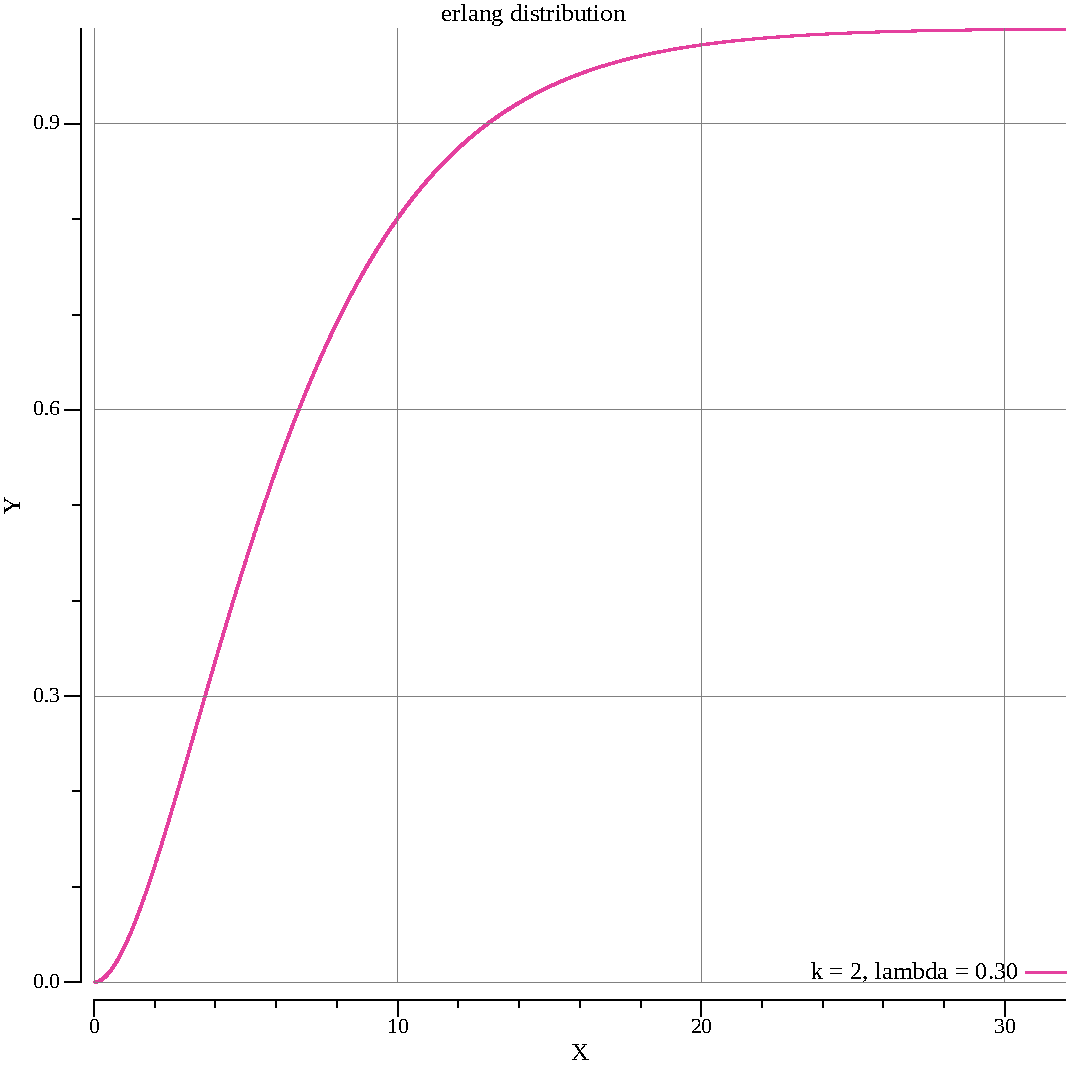
\includegraphics[width=1\linewidth]{assets/1}
    \caption{Калькулятор}
    \label{fig:1}
    \end{center}
\end{figure}

Далее по варианту 2 нужно произвести анализ влияния различных драйверов затрат на трудоемкость и длительность программного проекта.

В соответствии с вариантом используется промежуточная модель COCOMO. Количество строк кода --- 100 000. Были проварьированы параметры MODP – использование современных методов, TOOL – использование программных инструментов, ACAP – способности аналитика, PCAP – способности программиста от самых низкий значений до самых высоких. На основании полученных данных о трудоемкость и длительности были построены графики.

\begin{figure}[H]
    \begin{center}
    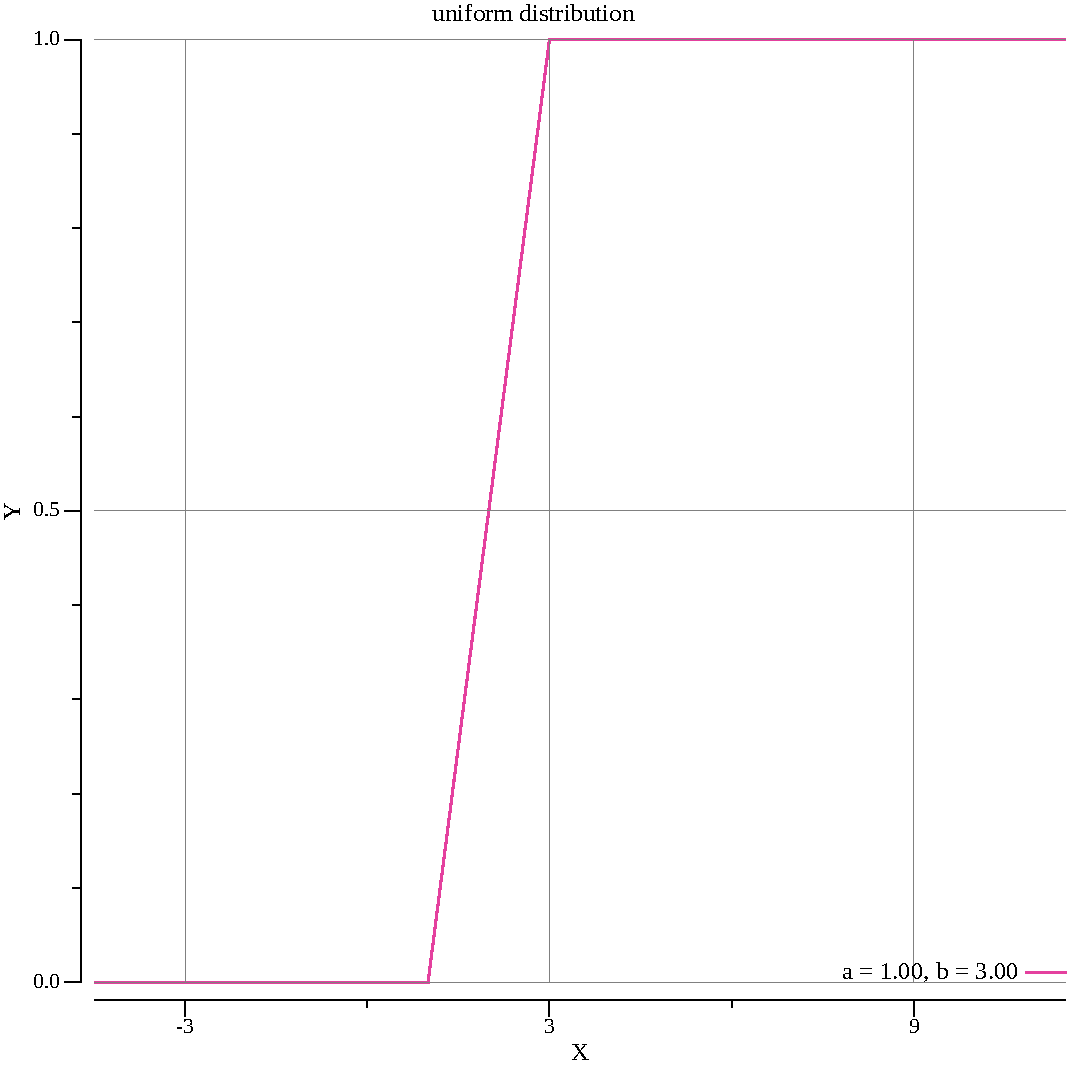
\includegraphics[width=1\linewidth]{assets/2}
    \caption{График трудоемкости}
    \label{fig:2}
    \end{center}
\end{figure}

\begin{figure}[H]
    \begin{center}
    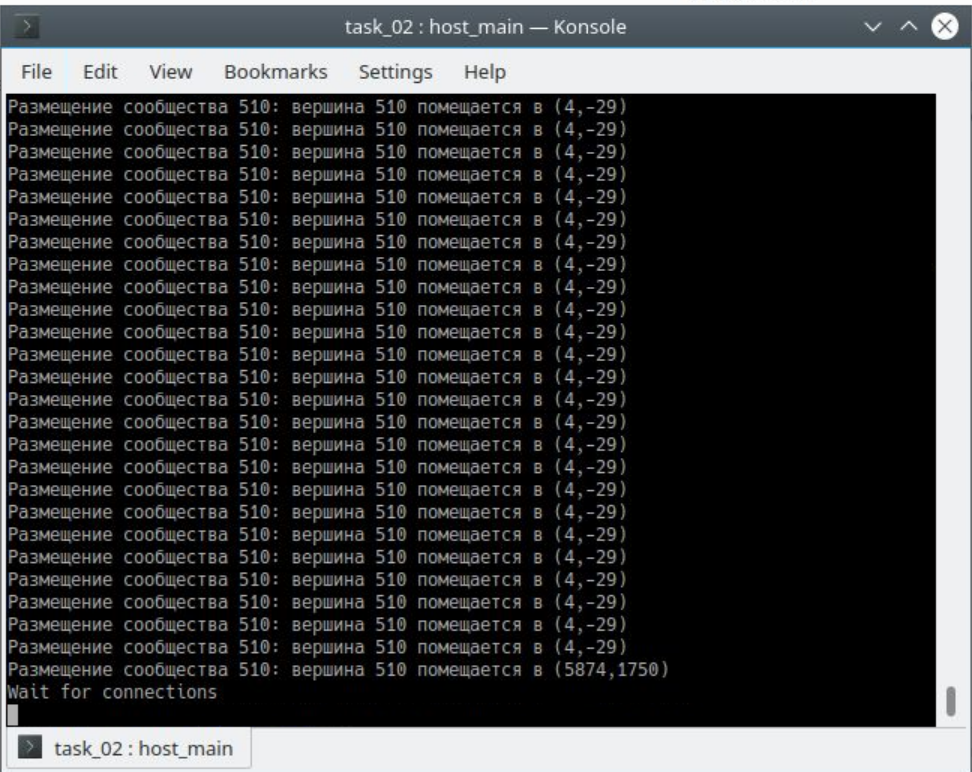
\includegraphics[width=1\linewidth]{assets/3}
    \caption{График длительности}
    \label{fig:3}
    \end{center}
\end{figure}

По результатам исследования можно сделать следующие выводы.

\begin{itemize}
	\item Способности персонала оказывают большее влияние как на трудоемкость, так и на длительность, чем степень автоматизации.
	\item MODP и TOOL одинаково влияют на параметры проекта.
	\item Очень низкие способности аналитика сильнее влияют на проект, чем очень низкие способности программиста.
	\item Очень высокие способности программиста сильнее влияют на проект, чем очень высокие способности аналитика.
	\item При необходимости сократить срок проекта, способности персонала повлияют больше, чем параметры среды.
\end{itemize}

Для высокой степени автоматизации (MODP и TOOL очень высокие), при требовании высокой надежности (RELY высокий) трудоемкость составляет 435.382 человеко-месяцев, длительность составляет 27.758 месяцев. При требовании чтобы не менее 70\% компонентов разрабатываемого ПО могло использоваться в режиме реального времени (TIME высокий) трудоемкость составляет 420.238 человеко-месяцев, длительность составляет 27.416 месяцев. Таким образом, требование к высокой надежности сильнее влияет на трудоемкость и длительность проекта.

В соответствии с вариантом был произведен расчет проекта. При разработке программного продукта его размер оценивается примерно в 55 KLOC. Этот проект будет представлять собой Web-систему, снабженную устойчивой серверной базой данных. Предполагается применение промежуточного варианта. Проект предполагает создание продукта средней сложности с номинальными требованиями по надежности, но с расширенной базой данных. Квалификация персонала средняя, однако способности аналитика высокие. 

Средняя зарплата разработчика в крупных городах сейчас составляет (по данным Хабр Карьеры) около 200 000 рублей.

\begin{figure}[H]
    \begin{center}
    \includegraphics[width=1\linewidth]{assets/4}
    \caption{Параметры проекта}
    \label{fig:4}
    \end{center}
\end{figure}

В результате были получены следующие параметры проекта. Трудозатраты составляют 267.715 месяцев, длительность составляет 23.413 месяцев. Стоимость проекта оценивается в 53 543 089 рублей.

\begin{figure}[H]
    \begin{center}
    \includegraphics[width=1\linewidth]{assets/5}
    \caption{Распределение работ по этапам жизненного цикла}
    \label{fig:5}
    \end{center}
\end{figure}

\begin{figure}[H]
    \begin{center}
    \includegraphics[width=1\linewidth]{assets/6}
    \caption{Распределение работ по видам деятельности WBS}
    \label{fig:6}
    \end{center}
\end{figure}

На основании полученных данных предлагается следующее распределение привлечения сотрудников.

\begin{figure}[H]
    \begin{center}
    \includegraphics[width=1\linewidth]{assets/7}
    \caption{Диаграмма привлечения сотрудников}
    \label{fig:7}
    \end{center}
\end{figure}
